% TEMPLATE.TEX
%
% Time-stamp: <2013-03-26 11:09 olenz>
%
% This is an extensively documented LaTeX file that shows how to
% produce a good-looking document with current LaTeX (11/2012).
%
% IMPORTANT!
%
%   Some obsolete commands and packages
% ----------|-------------------------------
% obsolete  |     Replacement in LATEX 2ε
% ----------|-------------------------------
%           | local            global/switch
% ----------|-------------------------------
% {\bf ...} | \textbf{...}     \bfseries
%     -     | \emph{...}       \em
% {\it ...} | \textit{...}     \itshape
%     -     | \textmd{...}     \mdseries
% {\rm ...} | \textrm{...}     \rmfamily
% {\sc ...} | \textsc{...}     \scshape
% {\sf ...} | \textsf{...}     \sffamily
% {\sl ...} | \textsl{...}     \slshape
% {\tt ...} | \texttt{...}     \ttfamily
%     -     | \textup{...}     \upshape
%
% DON'T USE \\ TO MAKE LINEBREAKS, INSTEAD JUST LEAVE A BLANK LINE!
%
\RequirePackage[l2tabu,orthodox]{nag} % turn on warnings because of bad style
\documentclass[a4paper,10pt,bibtotoc]{scrartcl}
%
\usepackage[bottom=3.5cm, top=3cm]{geometry}
\usepackage{subcaption}
\captionsetup[subfigure]{list=true, position=top}
\usepackage{float}
%%%%%%%%%%%%%%%%%%%%%%%%%%%%%%%%%%%%
% KOMA CLASSES
%%%%%%%%%%%%%%%%%%%%%%%%%%%%%%%%%%%%
%
% The class "scrartcl" is one of the so-called KOMA-classes, a set of
% very well done LaTeX-classes that produce a very European layout
% (e.g. titles with a sans-serif font).
%
% The KOMA classes have extensive documentation that you can access
% via the commands:
%   texdoc scrguide # in German
%   texdoc scrguien # in English
%
%
% The available classes are:
%
% scrartcl - for "articles", typically for up to ~20 pages, the
%            highest level sectioning command is \section
%
% scrreprt - for "reports", typically for up to ~200 pages, the
%            highest level sectioning command is \chapter
%
% scrbook  - for "books", for more than 200 pages, the highest level
%            sectioning command is \part.
%
% USEFUL OPTIONS
%
% a4paper  - Use a4 paper instead of the default american letter
%            format.
%
% 11pt, 12pt, 10pt
%          - Use a font with the given size.
%
% bibtotoc - Add the bibliography to the table of contents
%
% The KOMA-script classes have plenty of options to modify

% This allows to type UTF-8 characters like ä,ö,ü,ß
\usepackage[utf8]{inputenc}

\usepackage[T1]{fontenc}        % Tries to use Postscript Type 1 Fonts for better rendering
\usepackage{lmodern}            % Provides the Latin Modern Font which offers more glyphs than the default Computer Modern
\usepackage[intlimits]{amsmath} % Provides all mathematical commands
\usepackage{amssymb}
\usepackage{hyperref}           % Provides clickable links in the PDF-document for \ref
\usepackage{graphicx}            % Allow you to include images (like graphicx). Usage: \includegraphics{path/to/file}

% Allows to set units
\usepackage[ugly]{units}        % Allows you to type units with correct spacing and font style. Usage: $\unit[100]{m}$ or $\unitfrac[100]{m}{s}$

% Additional packages
\usepackage{url}                % Lets you typeset urls. Usage: \url{http://...}
\usepackage{breakurl}           % Enables linebreaks for urls
\usepackage{xspace}             % Use \xpsace in macros to automatically insert space based on context. Usage: \newcommand{\es}{ESPResSo\xspace}
\usepackage{xcolor}             % Obviously colors. Usage: \color{red} Red text
\usepackage{booktabs}           % Nice rules for tables. Usage \begin{tabular}\toprule ... \midrule ... \bottomrule
\usepackage{siunitx}


% Source code listings
\usepackage{listings}           % Source Code Listings. Usage: \begin{lstlisting}...\end{lstlisting}
\lstloadlanguages{python}
\definecolor{lightpurple}{rgb}{0.8,0.8,1}

\lstset{
stepnumber=1,
numbersep=5pt,
numberstyle=\small\color{black},
basicstyle=\ttfamily,
%keywordstyle=\color{black},
%commentstyle=\color{black},
%stringstyle=\color{black},
frame=single,
tabsize=4,
language = python,
backgroundcolor=\color{black!5}}

\usepackage{float}

\begin{document}

\titlehead{Simulation Methods in Physics I \hfill WS 2019/2010}
\title{Report for Worksheet 4: Thermostats}
\author{Markus Baur and David Beyer}
\date{\today}
%\publishers{Institute for Computational Physics, University of Stuttgart}
\maketitle

\tableofcontents

\section{Random Numbers}
\subsection{Linear Congruental Generator}
The code for this exercise can be found in the file ex\_4\_3\_random\_walk.py.
We implemented the linear congruental generator as a generator:
\begin{lstlisting}
def linear_congruental_generator():
    a = 1103515245
    c = 12345
    m = 2**32
    seed = 123647
    X = seed
    while True:
        X = (a*X + c) % m
        yield X/m
\end{lstlisting}
The declaration of the function as a generator allows us to use it as an iterator using the next command. 
In this case, the seed is just a fixed number (123647). Because we want a pseudo-random number in the interval $(0,1)$, the generator yields the quotient $X/m$.

To generate random walks consisting of $N$ steps starting from the starting point $x_0$, we wrote the following function:
\begin{lstlisting}
def random_walk(N, x0):
    ret = np.empty(N+1)
    ret[0] = x0
    k = linear_congruental_generator()
    for i in range(N):
        ret[i+1] = ret[i] + next(k) - 0.5
    return ret
\end{lstlisting}
This function has as its arguments the number of steps $N$ and the starting point $x_0$ and returns a NumPy array of length $N+1$ which contains the individual steps of the trajectory.
Every step, a random step size $\Delta x\in (-0.5,0.5)$ is added.
The random step size is generated using the function for the linear congruental generator defined above.
We could verify that the generated trajectory is always the same for a given seed.

To generate different trajectories, we use a different seed for every random walk.
One way to do this is to generate a seed from the current time:
\begin{lstlisting}
def linear_congruental_generator():
    a = 1103515245
    c = 12345
    m = 2**32
    seed = time.time_ns()
    X = seed
    while True:
        X = (a*X + c) % m
        yield X/m
\end{lstlisting}
The function time.time\_ns() returns the current time in nanoseconds as an integer.
A plot of ten different random walks which where generated using this method is shown in \autoref{fig:fig1}.
\begin{figure}[H]
	\centering
	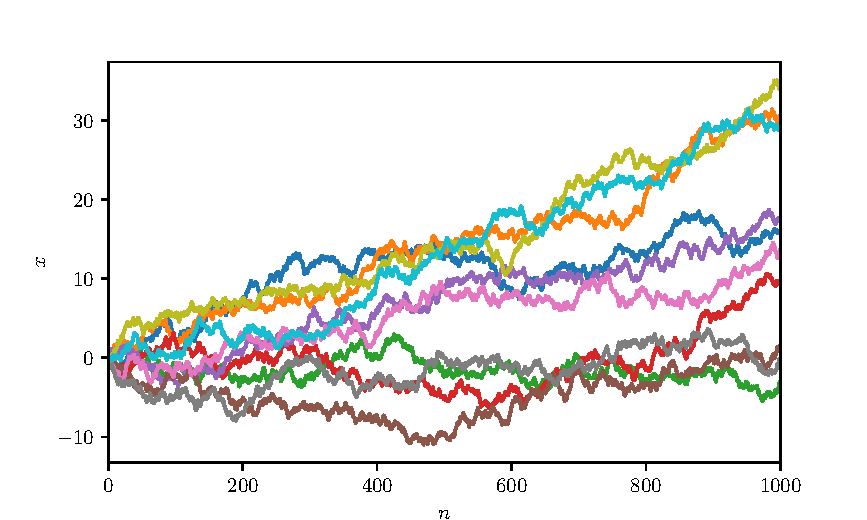
\includegraphics[width=\linewidth]{random_walk_time.pdf}
	\caption{Plot of ten different random walks with a seed generated from the current time.}
	\label{fig:fig1}
\end{figure}
\noindent Alternatively, we can create a random seed using os.urandom():
\begin{lstlisting}
def linear_congruental_generator():
    a = 1103515245
    c = 12345
    m = 2**32
    seed = int.from_bytes(os.urandom(10), sys.byteorder)
    X = seed
    while True:
        X = (a*X + c) % m
        yield X/m
\end{lstlisting}
A plot of ten different random walks which where generated using this method is shown in \autoref{fig:fig2}.
\begin{figure}[H]
	\centering
	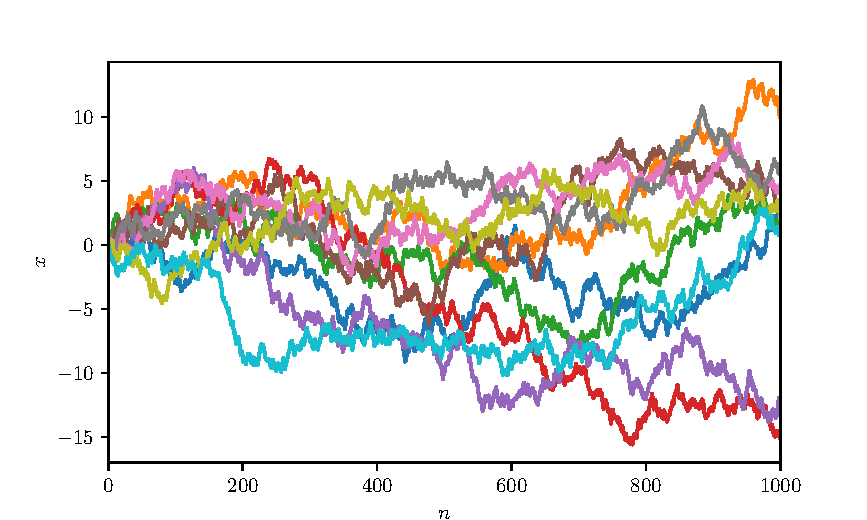
\includegraphics[width=\linewidth]{random_walk_os.pdf}
	\caption{Plot of ten different random walks with a seed generated using os.urandom().}
	\label{fig:fig2}
\end{figure}

\subsection{Box-Muller Transform}
\subsubsection{Gaussian Distribution}
The code for this exercise can be found in the file ex\_4\_3\_box\_muller.py. 
We again implemented a generator, it yields the random numbers which follow a Gaussian distribution and are generated using the Box-Muller transform:
\begin{lstlisting}
def box_muller(mean, sigma):
    while True:
        u1 = np.random.random()
        u2 = np.random.random()
        n1 = mean + sigma*np.sqrt(-2*np.log(u1))*np.cos(2*np.pi*u2)
        n2 = mean + sigma*np.sqrt(-2*np.log(u1))*np.sin(2*np.pi*u2)
        yield n1
        yield n2
\end{lstlisting}
The function has as its argument the desired mean and standard deviation of the Gaussian distribution. 
To generate the intial pair of random numbers, the NumPy implementation of the Mersenne Twister is used.
Then, the Box-Muller transform is performed.

A normalized histogram of $N=10000$ random numbers generated using the Box-Muller transform with mean of $\mu=1.0$ and standard deviation $\sigma = 4.0$ is shown in \autoref{fig:fig3}. 
Comparison with the analytical Gaussian distribution shows that the histogram approaches the analytical result quite closely.
\begin{figure}[H]
	\centering
	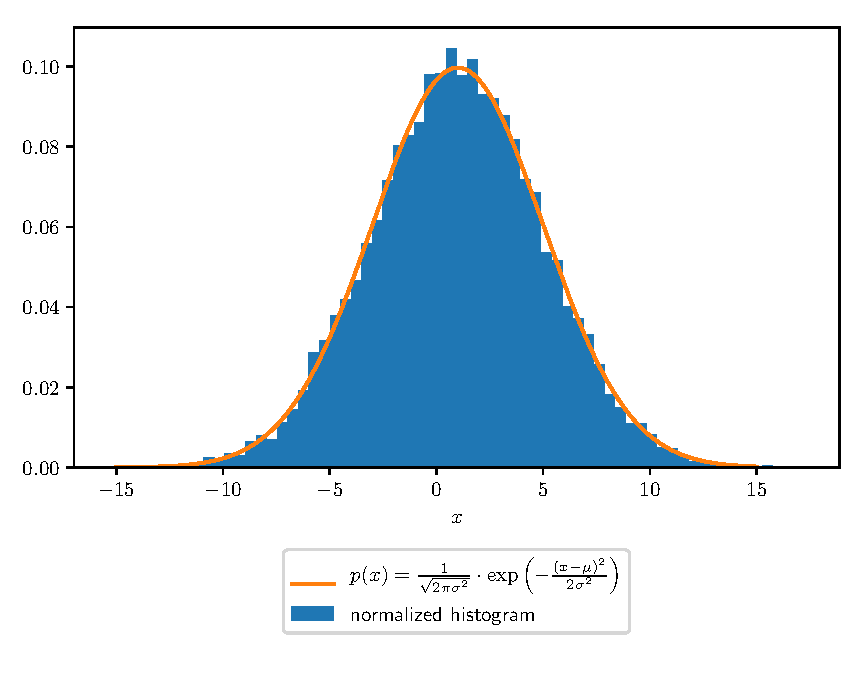
\includegraphics[width=\linewidth]{gaussian.pdf}
	\caption{Normalized histogram of $N=10000$ random numbers generated using the Box-Muller transform with mean of $\mu=1.0$ and standard deviation $\sigma = 4.0$. The analytical Gaussian distribution is also included.}
	\label{fig:fig3}
\end{figure}

\subsubsection{Maxwell-Boltzmann Distribution}
The distribution of particle speeds in a fluid can be described by the Maxwell-Boltzmann distribution.
To derive the Maxwell-Boltzmann distribution in three dimensions, we start with the canonical distribution for a classical fluid of $N$ particles, given by
\begin{align}
p\left(\{\mathbf{r}_i\}_{i=1,...,N},\{\mathbf{p}_i\}_{i=1,...,N}\right)\mathrm{d}\xi = \frac{1}{h^{3N}\cdot N!\cdot Z}\cdot\exp\left(-\beta\left(\sum_{i=1}^{N}\frac{\mathbf{p}_i^2}{2m} + V\left(\{\mathbf{r}_i\}_{i=1,...,N}\right)\right)\right)\mathrm{d}\xi.
\end{align}
Integrating over all particle coordinates results in the momentum distribution function
\begin{align}
p\left(\{\mathbf{p}_i\}_{i=1,...,N}\right)\mathrm{d}p = \mathcal{N}'\cdot\exp\left(-\beta\left(\sum_{i=1}^{N}\frac{\mathbf{p}_i^2}{2m} \right)\right)\mathrm{d}p
\end{align}
with a normalization $\mathcal{N}'$. 
Because the distribution factorizes and is the same for all particles, we may as well just look at the distribution of the $i$th particle, given by (we drop the index $i$):
\begin{align}
p\left(\mathbf{p}\right)\mathrm{d}p_x\mathrm{d}p_y\mathrm{d}p_z = \mathcal{N}\cdot\exp\left(-\beta\frac{\mathbf{p}^2}{2m}\right)\mathrm{d}p_x\mathrm{d}p_y\mathrm{d}p_z = \underbrace{\mathcal{N}m^3\cdot\exp\left(-\beta\frac{m\mathbf{v}^2}{2}\right)}_{=p\left(\mathbf{v}\right)}\mathrm{d}v_x\mathrm{d}v_y\mathrm{d}v_z.
\end{align}
$\mathcal{N}$ is again a normalization factor.
We can easily see that the individual components of the velocity are distributed according to a Gaussian distribution with mean $\mu= 0$ and standard deviation $\sigma = \left(\beta m\right)^{-\frac{1}{2}}$.
To obtain a distribution of the speed $v=\left|\mathbf{v}\right|$ we transform to spherical coordinates and integrate over the angles $\theta$ and $\phi$:
\begin{align}
\begin{split}
p\left(v\right)\mathrm{d}v &= \int_{\Omega}\,\mathcal{N}m^3\cdot\exp\left(-\beta\frac{mv^2}{2}\right)v^2\mathrm{d}v\mathrm{d}\Omega = 4\pi\mathcal{N}m^3v^2\cdot\exp\left(-\beta\frac{mv^2}{2}\right)\mathrm{d}v\\
&=\underbrace{4\pi\sqrt{\frac{\beta m}{2\pi}}^3v^2\cdot\exp\left(-\beta\frac{mv^2}{2}\right)}_{\text{Maxwell-Boltzmann distribution}}\mathrm{d}v.
\end{split}
\end{align}
Because the velocity components follow a Gaussian distribution, we can produce a Maxwell-Boltzmann distribution by calculating the distribution of the absolute values of threedimensional vectors with components that follow a Gaussian distribution.
Using the box\_muller generator defined above, this can be done in the following way:
\begin{lstlisting}
random_velocites = box_muller(0.0, 1.0)
v = [np.array([next(random_velocites),next(random_velocites),\
     next(random_velocites)]) for i in range(N_velocities)] 
v = np.array(v)
\end{lstlisting}
A normalized histogram can then be plotted using the histogram function of the matplotlib module:
\begin{lstlisting}
plt.hist(np.linalg.norm(v, axis=1), bins='auto',\
density = True, label='normalized histogram for $v$')
\end{lstlisting}
The obtained histogram and the analytical Maxwell-Boltzmann distribution are shown in \autoref{fig:fig4}, they are in close agreement
\begin{figure}[H]
	\centering
	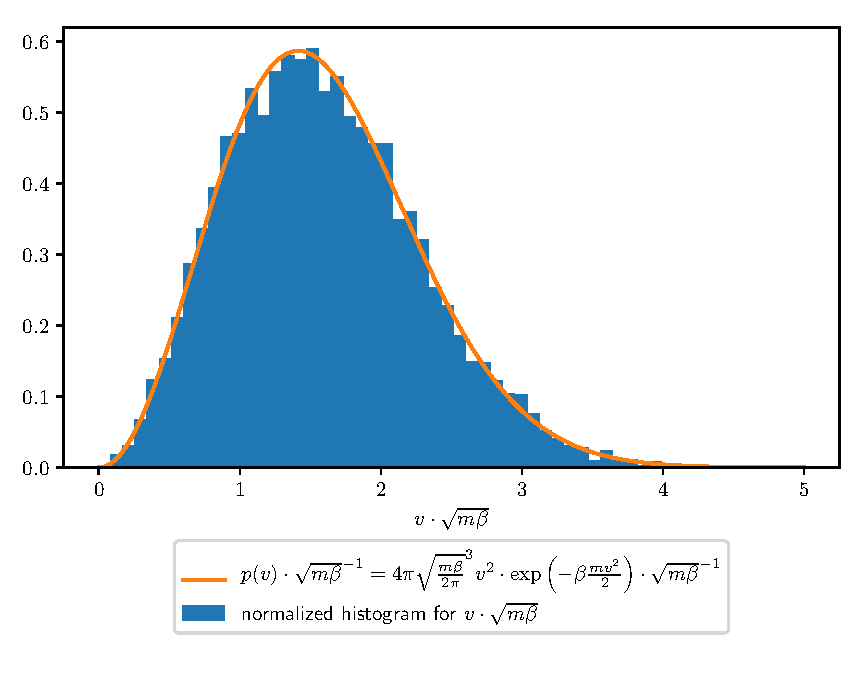
\includegraphics[width=\linewidth]{maxwell_boltzmann.pdf}
	\caption{Normalized histogram for the absolute value of $N=1000$ random 3-vectors $\mathbf{v}$ whose components are distributed according to a Gaussian distribution with mean $\mu=0.0$ and standard deviation $\sigma = 1.0$. The analytical Maxwell-Boltzmann distribution is also plotted.}
	\label{fig:fig4}
\end{figure}

\section{Langevin thermostat}
\subsection{Velocity-verlet step and temperature}
The velocity Verlet step for the Langevin thermostat is implemented in this way:
\begin{lstlisting}
def step_vv_langevin(x, v, f, dt, gamma):

    # update positions
    x += dt * v * (1 - dt * 0.5 * gamma) + 0.5 * dt * dt * f
    
    # half update velocity
    v = (v * (1 - 0.5 * gamma * dt)\
        + 0.5 * dt * f) / (1 + 0.5 * dt * gamma)
    
    #calculate new random force
    f = np.random.random_sample(np.shape(x))
    f -= 0.5
    f *= np.sqrt(12 * 2 * T * gamma / dt)

    # second half update of the velocity
    v += 0.5 * dt * f / (1 + 0.5 * dt * gamma)
    
    return x, v, f
\end{lstlisting}
The updating of the velocites is split into two steps, between the two sub-steps, the new random forces are calculated. 
The random forces follow a uniform distribution which is generated using the random\_sample function of NumPy.random.
To compute the current temperature using the equipartition theorem, the function compute\_temperature is implemented:
\begin{lstlisting}
def compute_temperature(v):
    ret = compute_energy(v) * 2. / (NDIM * N)
    return ret

def compute_energy(v):
    return (v * v).sum() / 2.
\end{lstlisting}
The function uses the kinetic energy, which is calculated using compute\_energy to calculate the temperature.
\subsection{Temperature and velocity distribution}
In \autoref{fig:fig5} we can see the time evolution of the Temperature.
The temperature fluctuates around the value $T=0.3*T_0$ ($T_0$ is the temperature scale) which is used in the simulation. 
In contrast to the velocity rescaling thermostat which was used on the last sheet, the temperature is actually not constant but fluctuates around a constant value, this is what we would expect from the canonical ensemble.
\begin{figure}[H]
	\centering
	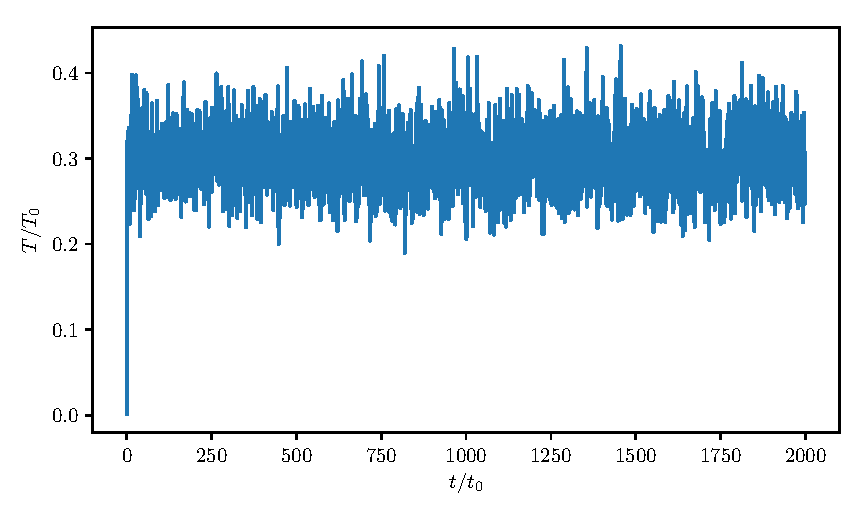
\includegraphics[width=\linewidth]{temperature.pdf}
	\caption{Time evolution of the temperature $T$ (in units of $T_0$.}
	\label{fig:fig5}
\end{figure}
\autoref{fig:fig6} shows the normalized histogram for the (dimensionless) absolute value of the velocity $v\cdot \sqrt{m\beta}$ which was obtained by computing the histogram over all all particle velocites at all times.
A comparison with the corresponding Maxwell-Boltzmann distribution shows, that the two are approximately equal.
\begin{figure}[H]
	\centering
	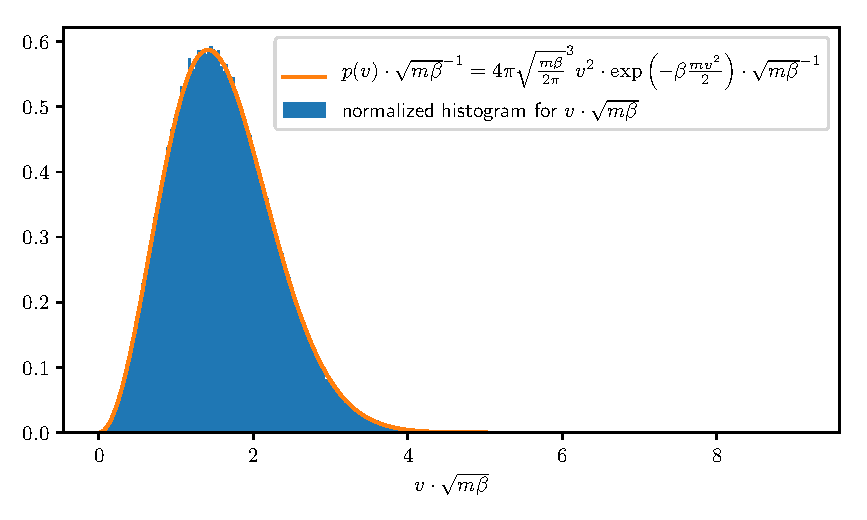
\includegraphics[width=\linewidth]{maxwell_boltzmann_langevin.pdf}
	\caption{Normalized histogram of the velocity $v$ and corresponding Maxwell-Boltzmann distribution.}
	\label{fig:fig6}
\end{figure}


\section{Diffusion coefficients}
The code for this section can be found in the file analysis.py.
\subsection{Mean square displacement}
To calculate the mean squared displacement, we implemented the function MSD:
\begin{lstlisting}
def MSD(traj):
    dx = np.zeros((timesteps, N))
    error = np.zeros(timesteps)
    for l in range(N):
        for i in range(1, timesteps):
            for j in range(int(timesteps/(i + 1))):
                start = (i + 1) * j
                end = (i + 1) * (j + 1) - 1
                for k in range(traj.shape[2]):
                    dx[i, l] += np.power(traj[end, l, k]\
                    - traj[start, l, k], 2)
            dx[i, l] /= int(timesteps/(i + 1))
            error[i] = standard_error(dx[i,:])
        
        dx_average = np.average(dx, axis=1)
    return dx_average, error
\end{lstlisting}
This function has as its input an array which contains all of the particle trajectories. 
The function calculates the mean squared displacement for each trajectory separately in the way it is defined on the worksheet. 
Furthermore, the estimator of the standard error is calculated for each value of $\Delta t$. 
Because the trajectories of the individual particles are uncorrelated, we can simply use the formula
\begin{align}
\epsilon(A) = \sqrt{\frac{1}{N(N-1)}\cdot \left(\sum_{i=1}^{N} A_i^2 - \left(\sum_{i=1}^{N} A_i\right)^2\right)}.
\end{align}
In order to calculate the estimator of the standard error for a series of uncorrelated values, we implemented the function standard\_error:
\begin{lstlisting}
def standard_error(x):
    N = len(x)
    ret = np.dot(x,x) - np.sum(x)**2 / N
    ret /= N * (N - 1)
    ret = np.sqrt(ret)
    return ret
\end{lstlisting}
This function is then used in MSD. 
The function MSD finally returns the average mean squared displacement and the estimator of the standard error.
\autoref{fig:fig7} shows a plot of the MSD which was obtained from the simulated trajectories.
Errorbars for the estimator of the standard error are also shown.
A linear fit to the MSD over the first 1000 time steps gives a value of 
\begin{align}
D_\text{MSD, fit} \approx 0.3599.
\end{align}
The theoretical value from the Einstein relation is
\begin{align}
D = \frac{k_\mathrm{B}T}{\gamma} = \frac{0.3}{0.8} = 0.375.
\end{align}
\begin{figure}[H]
	\centering
	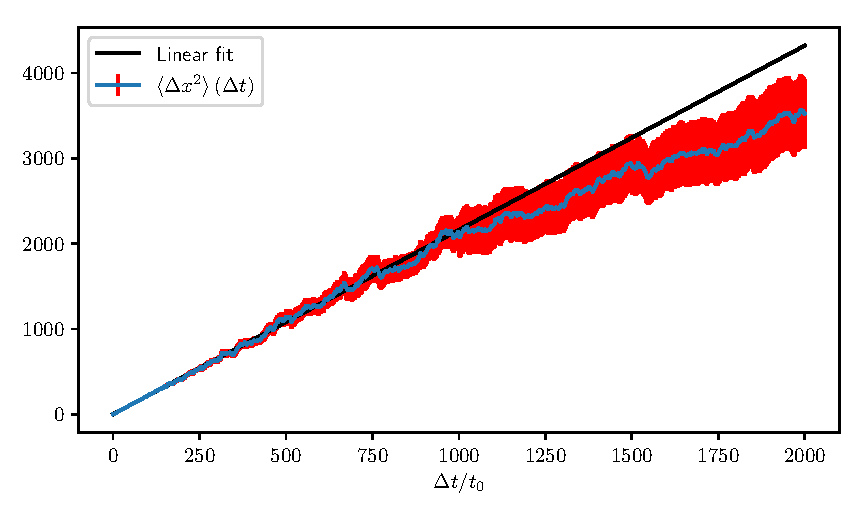
\includegraphics[width=\linewidth]{msd.pdf}
	\caption{Plot of the mean square displacement (with errorbars). The linear fit over the first 1000 time steps is also plotted.}
	\label{fig:fig7}
\end{figure}
\autoref{fig:fig7b} shows the mean square displacement for short times.
We can see that in the beginning, the mean squared displacement is growing quadratically, this is indicative of ballistic motion:
Because between collisions, the Brownian particles move with a constant velocity, the behaviour for short times resembles the motion of free particles with a mean displacement which is growing linearly in time.
\begin{figure}[H]
	\centering
	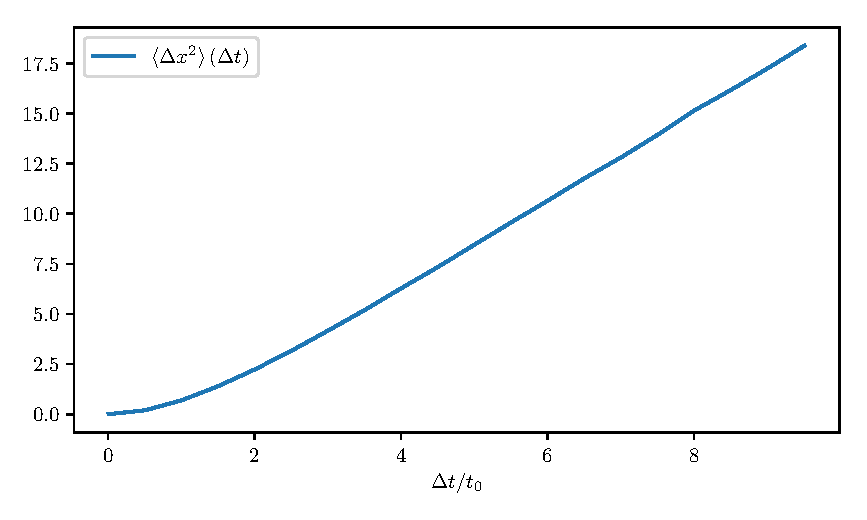
\includegraphics[width=\linewidth]{msd_short_times.pdf}
	\caption{Plot of the mean square displacement for a short time interval.}
	\label{fig:fig7b}
\end{figure}

\subsection{VACF}
To calculate and plot the velocity autocorrelation function, we implemented the function VACF:
\begin{lstlisting}
def VACF(v):
    v = v.T
    r = np.zeros(timesteps * 2 - 1)
    for d in range(v.shape[0]):  # number of dimensions
        for part in range(v.shape[1]):  # for each particle
            r += np.convolve(v[d][part], np.flip(v[d][part]),\
            'full')
    r /= (len(ts)*v.shape[0]*v.shape[1])
    plt.plot(np.linspace(-0.5*timesteps, 0.5*timesteps,\
    len(r)), r/0.3)
    plt.xlabel(r'$t/t_0$')
    plt.ylabel(r'VACF $\langle v(0)v(t)\rangle\
    \cdot \frac{m}{k_\mathrm{B} T}$')
    plt.tight_layout()
    plt.xlim((-30.0, 30.0))
    plt.show()

    D = 0.5 * np.trapz(r,dx=0.5)
    print(D)
    
    param, cov = curve_fit(vacf_exp, ts, r[timesteps - 1:])
    print(*param)
\end{lstlisting}
The function has as its input an array of all velocities.
First, the function calculates the averaged velocity autocorrelation function, by averaging the velocity autocorrelation functions of the individiual trajectories.
The autocorrelation functions are calculated using the NumPy function convolve. 
In order to get the correct normalization, it is important to divide the computed convolution by the number of time steps.
Plots of the computed autocorrelation function are shown in \autoref{fig:fig8} and \autoref{fig:fig9}.
We can see that the velocity autocorrelation function is symmetric, has its maximum at $t=0$ and rapidly falls off to zero.
Indeed, from the analytical results we would expect an exponential decay.
To obtain the diffusion coefficient via the Green-Kubo relation, we have to integrate the velocity correlation function.
We implemented two different ways to do this integration.
First, we calculate the integral numerically, using the NumPy function np.trapz. 
The result we obtained this way is
\begin{align}
D_\text{Green-Kubo, numerical integral} \approx 0.2933.
\end{align}
Alternatively, we fitted an exponential function $a\cdot \exp (-b\cdot t)$ to the velocity autocorrelation function, the obtained fit parameters were
\begin{align}
a \approx 0.3002\\
b \approx 0.7987.
\end{align}
By analytically integrating the exponential function and plugging in the fit parameters, we then obtain
\begin{align}
D_\text{Green-Kubo, fit} \approx 0.3758.
\end{align}
This value is actually by far the closest to the theoretical value given above. 
In contrast, the value obtained by numerically integrating seems to be the worst, this can be explained by the fact that we did not actually integrate over $[0,\infty)$ but only over a finite interval, this leads to a value that is much smaller than the theoretical expectation.
\begin{figure}[H]
	\centering
	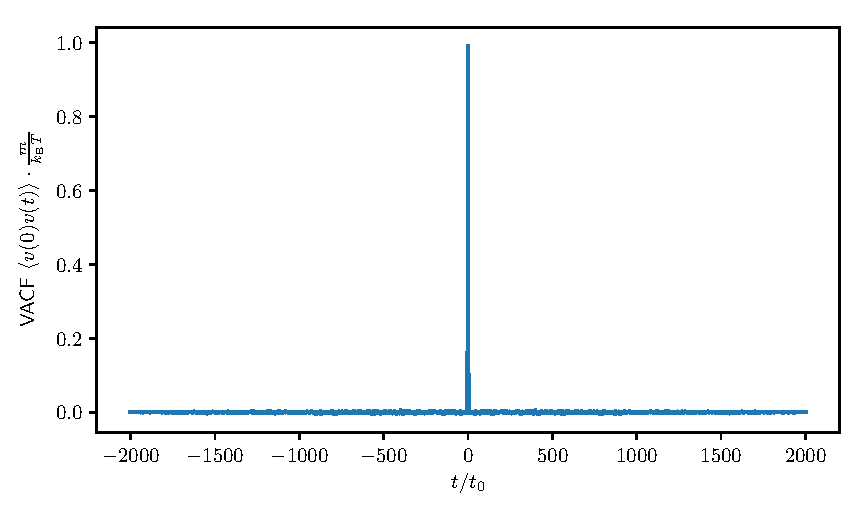
\includegraphics[width=\linewidth]{vacf.pdf}
	\caption{Numerically computed velocity autocorrelation function (VACF).}
	\label{fig:fig8}
\end{figure}

\begin{figure}[H]
	\centering
	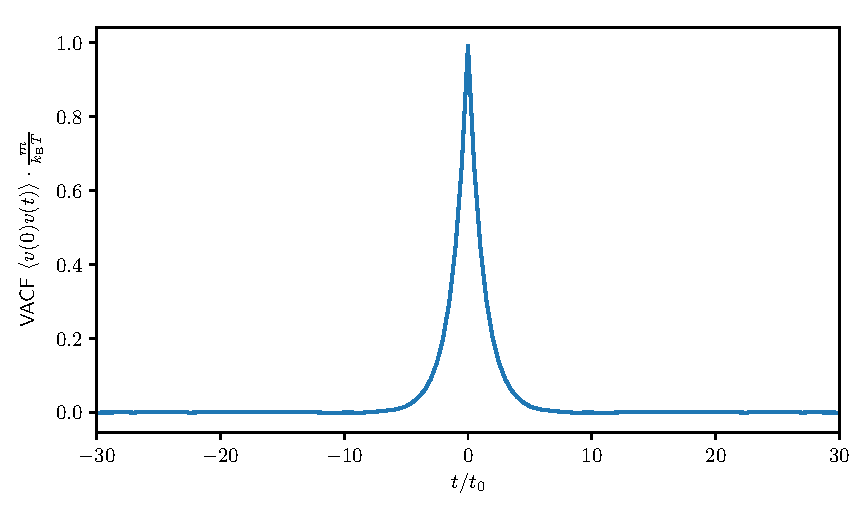
\includegraphics[width=\linewidth]{vacf_zoom.pdf}
	\caption{Numerically computed velocity autocorrelation function (VACF).}
	\label{fig:fig9}
\end{figure}

\section{Diffusion equation}
The initial positions, velocites and forces are set up in the following way:
\begin{lstlisting}
# Initial positions (1 coordinate per particle)
x = np.zeros((N,NDIM))

# Initial velocities
v = np.random.normal(0.0, np.sqrt(args.T), (N,NDIM))

# Initial forces
f = np.zeros((N,NDIM))
\end{lstlisting}
The initial velocites are drawn from a Gaussian distribution of mean 0 and standard deviation $\sigma = \sqrt{k_\mathrm{B}T/m}$ ($=\sqrt{T}$ in the units which are used).
The velocity Verlet step for the Langevin thermostat is exactly the same as in the previous exercises.

The analytical solution for the given inital condition is given by
\begin{align}
P(x, t) = \frac{1}{2\sqrt{\pi D t}}\cdot \exp\left(-\frac{x^2}{4Dt}\right)
\end{align}
which is just a Gaussian distribution with variance $\sigma^2 = 2Dt$.
For a given temperature $T$ and friction coefficient $\gamma$, the diffusion coefficient $D$ can be calculated using the Einstein relation
\begin{align}
D = \frac{k_\mathrm{B}T}{\gamma}
\end{align}
which is a special case of the fluctuation-disspiation theorem.
The function which computes and plots the histogram of the particle positions has the following form:
\begin{lstlisting}
def plot(pos, time, color, T, gamma):
    # Boundaries of the histogram (make them symmetric)
    hist_range = max(-np.amin(pos), np.amax(pos))

    # Sample positions into a histogram
    H = np.histogram(pos, bins=200, density=True)

    # Calculate bin centers
    bin_centers = (H[1][:-1] + H[1][1:]) / 2
    plt.plot(bin_centers, H[0])

    # Plot the analytical solution
    D = T / gamma
    x = np.linspace(-10.0, 10.0, 1000)
    plt.plot(x, gaussian_distribution(x, 0.0, np.sqrt(2 * D * time)))
\end{lstlisting}
Furthermore, the analytical solution is also plotted.
\autoref{fig:figdiffusion1} - \autoref{fig:figdiffusion3} the computed histogram as well as the analytical solution for three different times.
We can see that the numerical histogram fluctuates around the analytical solution.

\begin{figure}[H]
	\centering
	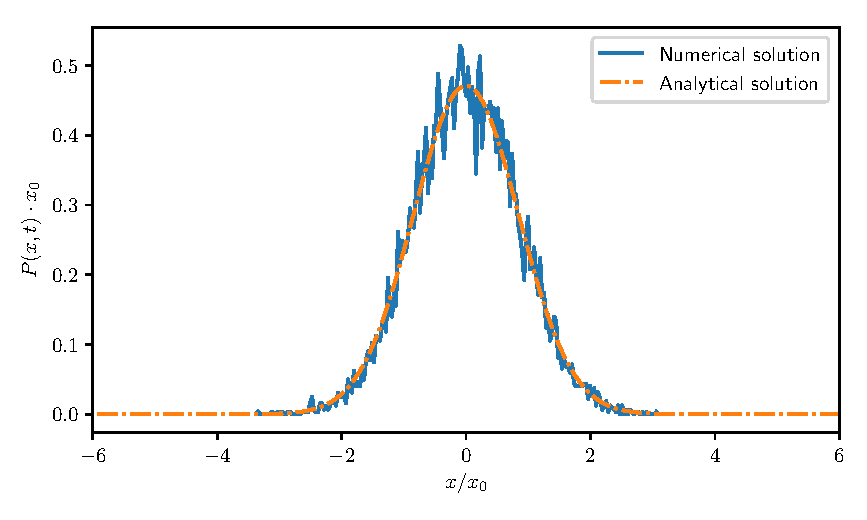
\includegraphics[width=\linewidth]{diffusion300.pdf}
	\caption{Calculated histogram of the numerical trajectories as well as the analytical solution for $\gamma = 10$ and $T=1.2$ after 300 time steps.}
	\label{fig:figdiffusion1}
	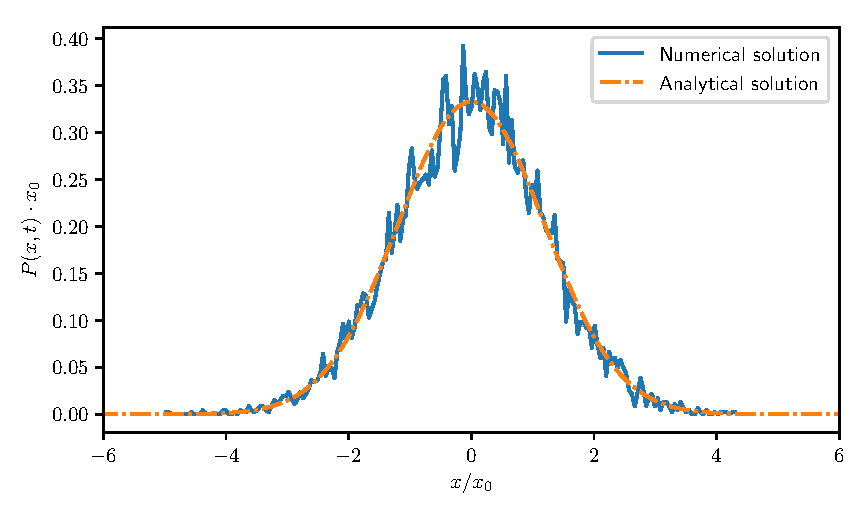
\includegraphics[width=\linewidth]{diffusion600.pdf}
	\caption{Calculated histogram of the numerical trajectories as well as the analytical solution for $\gamma = 10$ and $T=1.2$ after 600 time steps.}
	\label{fig:figdiffusion2}
\end{figure}

\begin{figure}[H]
	\centering
	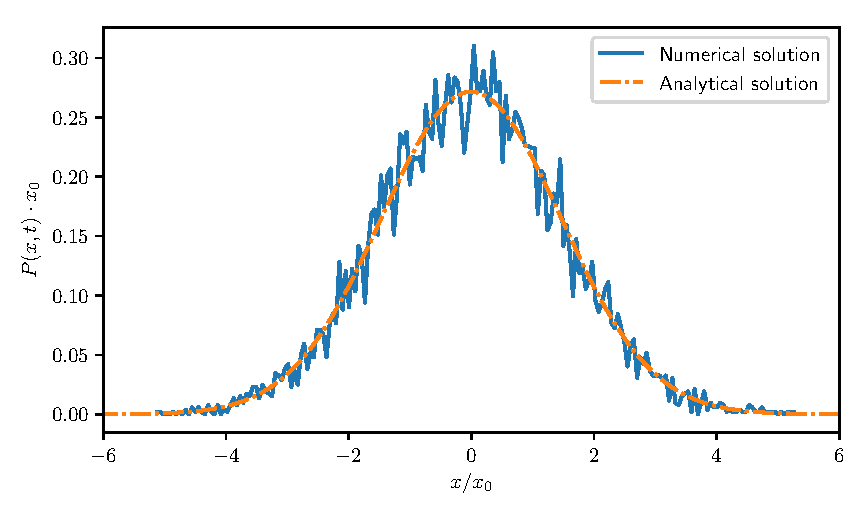
\includegraphics[width=\linewidth]{diffusion900.pdf}
	\caption{Calculated histogram of the numerical trajectories as well as the analytical solution for $\gamma = 10$ and $T=1.2$ after 900 time steps.}
	\label{fig:figdiffusion3}
\end{figure}


\end{document}
